\documentclass[aspectratio=169,11pt]{beamer}

\usetheme{Boadilla}
\useinnertheme{rectangles}
\usefonttheme{professionalfonts}
\setbeamertemplate{navigation symbols}{}
\setbeamertemplate{blocks}[rounded][shadow=false]
\setbeamersize{text margin left=9mm,text margin right=9mm}

\usepackage{amsmath,amssymb}
\usepackage{booktabs}
\usepackage{graphicx}
\usepackage{tikz}
\usetikzlibrary{arrows.meta,positioning,fit,calc}
\usepackage{xcolor}

\graphicspath{{figs/}}

\definecolor{anchorblue}{RGB}{34,94,168}
\definecolor{quantred}{RGB}{168,72,34}
\definecolor{servergold}{RGB}{184,134,11}
\definecolor{buffergreen}{RGB}{44,122,95}
\definecolor{slate}{RGB}{30,44,58}
\definecolor{paperbg}{RGB}{248,247,243}
\definecolor{textgray}{RGB}{73,83,92}

\setbeamercolor{background canvas}{bg=paperbg}
\setbeamercolor{normal text}{fg=slate}
\setbeamercolor{structure}{fg=anchorblue}
\setbeamercolor{frametitle}{bg=slate, fg=white}
\setbeamercolor{title}{fg=slate}
\setbeamercolor{block title}{bg=anchorblue!16, fg=slate}
\setbeamercolor{block body}{bg=white, fg=slate}
\setbeamercolor{alerted text}{fg=quantred}
\setbeamerfont{title}{series=\bfseries, size=\Large}
\setbeamerfont{frametitle}{series=\bfseries, size=\large}
\setbeamerfont{block title}{series=\bfseries}

\setbeamertemplate{footline}{%
  \leavevmode%
  \hbox{%
    \begin{beamercolorbox}[wd=.82\paperwidth,ht=2.8ex,dp=1.2ex,leftskip=1em]{author in head/foot}%
      \color{textgray}\footnotesize Anchor-Guided Dequantization for Federated Learning
    \end{beamercolorbox}%
    \begin{beamercolorbox}[wd=.18\paperwidth,ht=2.8ex,dp=1.2ex,rightskip=1em plus1fil]{date in head/foot}%
      \color{textgray}\footnotesize \insertframenumber/\inserttotalframenumber
    \end{beamercolorbox}%
  }%
}

\title{Anchor-Guided Dequantization\\for Federated Learning}
\subtitle{Repairing low-bit client updates with full-precision anchors}
\author{Jacob Simmons \and Owen Strength}
\date{Auburn University\\COMP 5970/6970 Course Project}

\begin{document}

\begin{frame}[plain]
  \vspace{1.0em}
  {\color{anchorblue}\rule{\textwidth}{2pt}}

  \vspace{0.9em}
  {\LARGE\bfseries Anchor-Guided Dequantization}\\[0.25em]
  {\Large\bfseries for Federated Learning}

  \vspace{0.5em}
  {\large Repairing low-bit client updates with full-precision anchors}

  \vspace{1.1em}
  {\color{anchorblue!65}\rule{\textwidth}{0.8pt}}

  \vspace{1.0em}
  \textbf{Jacob Simmons} (\texttt{jss0112@auburn.edu})\\
  \textbf{Owen Strength} (\texttt{ods0005@auburn.edu})\\
  Auburn University\\
  COMP 5970/6970 Course Project

  \vfill
  \small
  \textcolor{textgray}{CIFAR-10 \quad 10 clients \quad INT2 / INT4 / INT8 \quad server-side CorrectionNet}
\end{frame}

\begin{frame}{Problem Setting}
\small
\begin{columns}[T,totalwidth=\textwidth]
\column{0.50\textwidth}
\begin{block}{Standard FL assumption}
FedAvg works well when uploaded client updates are already comparable and can
be averaged directly.
\end{block}

\vspace{0.2em}
\begin{block}{What changes here}
Clients are \textbf{bit-width heterogeneous}.
\begin{itemize}\setlength{\itemsep}{0.15em}
  \item Anchor clients upload \textbf{FP32} deltas.
  \item Constrained clients upload \textbf{INT8 / INT4 / INT2} deltas.
  \item The server averages \emph{clean} and \emph{biased} updates together.
\end{itemize}
\end{block}

\column{0.46\textwidth}
\begin{block}{Failure mode}
Quantization error is not just random noise.
\begin{itemize}\setlength{\itemsep}{0.15em}
  \item Low-bit updates lose magnitude information.
  \item With very few levels, signs cancel and the average collapses.
  \item The global model absorbs that distortion every round.
\end{itemize}
\end{block}

\vspace{0.1em}
\begin{alertblock}{Bias at the server}
If the constrained upload is a distorted version of the full-precision update,
then averaging clean and quantized deltas pushes the server in the wrong
direction.
\end{alertblock}
\end{columns}
\end{frame}

\begin{frame}{Why Existing Fixes Are Not Enough}
\small
\begin{columns}[T,totalwidth=\textwidth]
\column{0.48\textwidth}
\begin{block}{FedAvg}
\begin{itemize}
  \item No correction step at all.
  \item Assumes averaging cancels quantization noise; breaks hardest at INT2.
\end{itemize}
\end{block}

\vspace{0.2em}
\begin{block}{FedShift}
\begin{itemize}
  \item One global anchor-based shift per round.
  \item Strong near-IID baseline, but still one target for everyone.
\end{itemize}
\end{block}

\column{0.48\textwidth}
\begin{block}{ProWD}
\begin{itemize}
  \item Learned residual MLP, but trained on the current round only.
  \item Pulls every constrained client toward the same mean anchor target.
\end{itemize}
\end{block}

\vspace{0.2em}
\begin{block}{AGD-Smart}
\begin{itemize}
  \item Replay buffer plus direct anchor supervision.
  \item Client-specific matching instead of one global target.
  \item Blended correction when non-IID structure matters.
\end{itemize}
\end{block}
\end{columns}

\vspace{0.2em}
\centering
\footnotesize AGD-Smart is the only variant that is both persistent and
client-specific.
\end{frame}

\begin{frame}{Method Overview}
\begin{center}
\resizebox{0.78\linewidth}{!}{\providecommand{\methoddiagramfont}{\small}

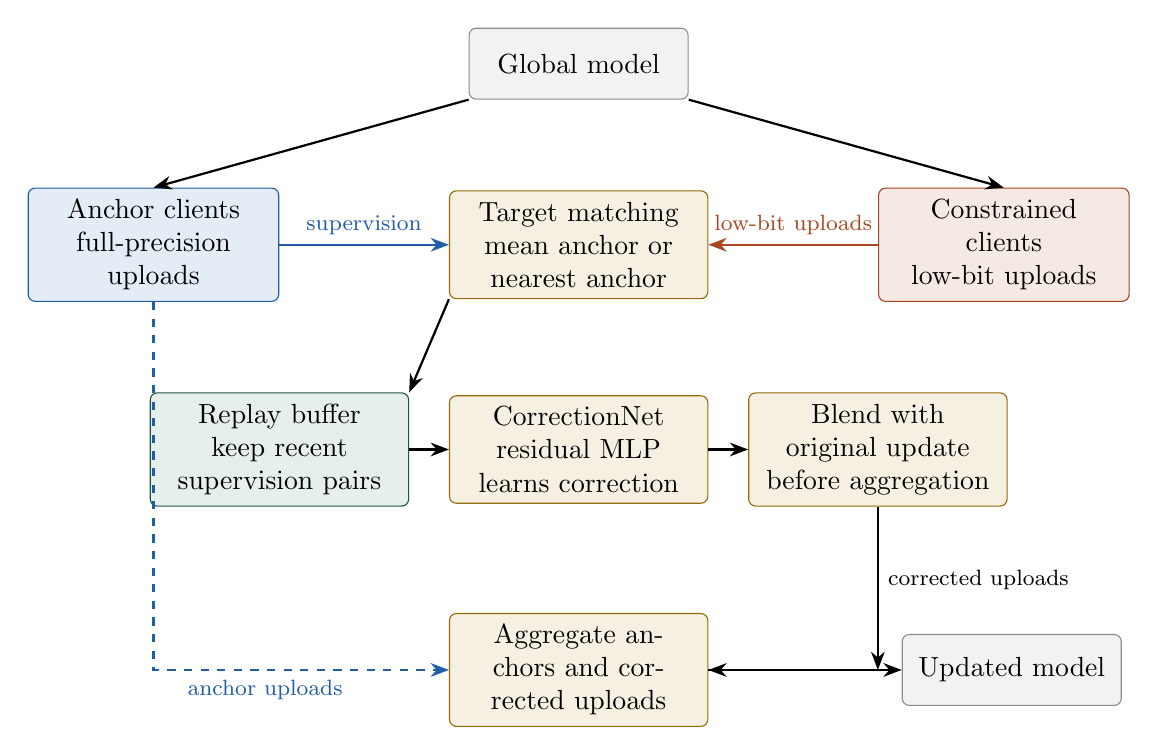
\begin{tikzpicture}[
  >=Stealth,
  font=\methoddiagramfont,
  box/.style={
    draw,
    rounded corners=2.5pt,
    align=center,
    inner sep=4pt,
    minimum height=9mm
  },
  model/.style={box, fill=black!5, draw=black!45, text width=2.5cm},
  anchorbox/.style={box, fill=anchorblue!12, draw=anchorblue, text width=2.9cm},
  quantbox/.style={box, fill=quantred!12, draw=quantred, text width=2.9cm},
  serverbox/.style={box, fill=servergold!12, draw=servergold!80!black, text width=3.0cm},
  bufferbox/.style={box, fill=buffergreen!12, draw=buffergreen!70!black, text width=3.0cm}
]

\node[model] (global) at (0, 0) {Global model};

\node[anchorbox] (anchors) at (-5.4, -2.3) {Anchor clients\\full-precision uploads};
\node[serverbox] (targets) at (0, -2.3) {Target matching\\mean anchor or nearest anchor};
\node[quantbox] (quantized) at (5.4, -2.3) {Constrained clients\\low-bit uploads};

\node[bufferbox] (replay) at (-3.8, -4.9) {Replay buffer\\keep recent supervision pairs};
\node[serverbox] (corrnet) at (0, -4.9) {CorrectionNet\\residual MLP learns correction};
\node[serverbox] (blend) at (3.8, -4.9) {Blend with original update\\before aggregation};

\node[serverbox] (agg) at (0, -7.7) {Aggregate anchors and corrected uploads};
\node[model] (next) at (5.5, -7.7) {Updated model};

\coordinate (aggleft) at ([xshift=-0.8cm]agg.west);
\coordinate (aggright) at ([xshift=0.8cm]agg.east);
\coordinate (blenddrop) at (blend.south |- aggright);

\draw[->, thick] (global.south west) -- (anchors.north);
\draw[->, thick] (global.south east) -- (quantized.north);
\draw[->, thick, anchorblue] (anchors.east) -- node[above, font=\footnotesize] {supervision} (targets.west);
\draw[->, thick, quantred] (quantized.west) -- node[above, font=\footnotesize] {low-bit uploads} (targets.east);
\draw[->, thick] (targets.south west) -- (replay.north east);
\draw[->, thick] (replay.east) -- (corrnet.west);
\draw[->, thick] (corrnet.east) -- (blend.west);
\draw[->, thick] (blend.south) -- node[pos=0.45, right, font=\footnotesize] {corrected uploads} (blenddrop);
\draw[->, thick] (blenddrop) -- (aggright) -- (agg.east);
\draw[->, thick, anchorblue, dashed] (anchors.south) |- node[pos=0.74, below, font=\footnotesize] {anchor uploads} (aggleft) -- (agg.west);
\draw[->, thick] (agg.east) -- (next.west);

\end{tikzpicture}
}
\end{center}
\end{frame}

\begin{frame}{What Happens Each Round}
\begin{columns}[T,totalwidth=\textwidth]
\column{0.52\textwidth}
\textbf{1. Collect two kinds of updates}
\begin{itemize}
  \item Anchors send clean FP32 deltas $\Delta w_a^{\mathrm{fp}}$.
  \item Constrained clients send quantized deltas $\Delta w_j^q$.
\end{itemize}

\vspace{0.5em}
\textbf{2. Build targets for constrained clients}
\begin{itemize}
  \item Baseline mode: target the \emph{mean} anchor delta.
  \item Smart mode: choose the anchor whose update points in the most similar direction.
\end{itemize}

\column{0.44\textwidth}
\textbf{3. Train on buffered supervision}
\begin{itemize}
  \item Store $(\Delta w_j^q,\Delta w_j^{\mathrm{target}})$ pairs.
  \item Keep the most recent \textbf{10 rounds}.
  \item Normalize buffered inputs with a scalar $z$-score before training.
\end{itemize}

\vspace{0.5em}
\textbf{4. Correct, blend, aggregate}
\begin{itemize}
  \item Apply the learned map to each constrained delta.
  \item Blend corrected and original directions when needed.
  \item Aggregate anchors plus corrected constrained updates.
\end{itemize}
\end{columns}
\end{frame}

\begin{frame}{CorrectionNet and Training Objective}
\begin{columns}[T,totalwidth=\textwidth]
\column{0.50\textwidth}
\begin{block}{CorrectionNet}
\begin{itemize}
  \item One encoder layer
  \item Three residual blocks
  \item Zero-initialized decoder
\end{itemize}
Zero-init matters: training starts from an identity map, so the network learns
\emph{bias correction} instead of a full rewrite of the update.
\end{block}

\column{0.46\textwidth}
\begin{block}{Loss}
\begin{itemize}
  \item Reconstruction term: make the corrected upload look like the chosen anchor target.
  \item Optional distillation term: make the repaired update produce similar logits on a server validation split.
  \item $\tau=4$ in the reported settings.
\end{itemize}
\end{block}
\end{columns}
\end{frame}

\begin{frame}{Why Warmup Matters}
\begin{columns}[T,totalwidth=\textwidth]
\column{0.52\textwidth}
\begin{block}{Warmup}
For the first \textbf{5 rounds}, the server trains CorrectionNet but does not
apply correction yet.
\begin{itemize}
  \item The replay buffer fills with real supervision pairs.
  \item The untrained network cannot damage early optimization.
  \item Correction activates only after there is enough signal to use.
\end{itemize}
\end{block}

\column{0.44\textwidth}
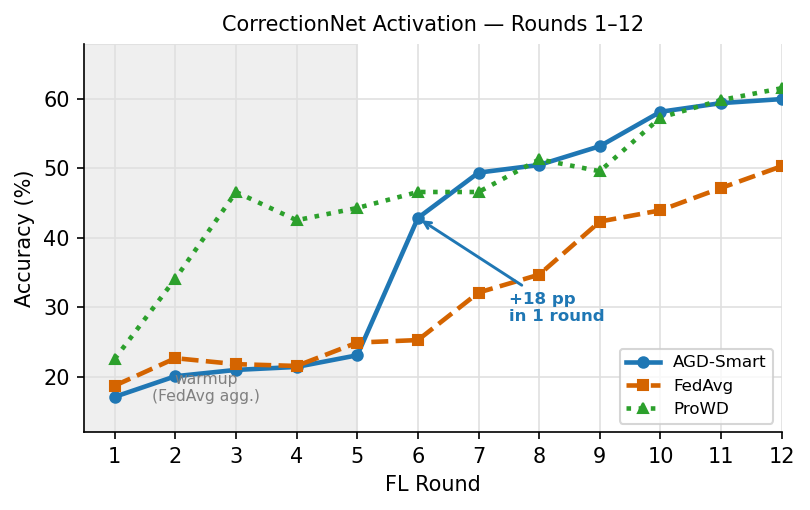
\includegraphics[width=0.92\linewidth]{int2_warmup.png}

\vspace{0.4em}
\small
\textbf{Interpretation:} the jump appears exactly when correction turns on after
warmup.
\end{columns}
\end{frame}

\begin{frame}{Why Blending Matters}
\begin{columns}[T,totalwidth=\textwidth]
\column{0.52\textwidth}
\begin{block}{Blended correction}
Use \textbf{80\% corrected update + 20\% original update} in the smart
configuration.
\end{block}

\column{0.44\textwidth}
\small
In the smart configuration, $\beta=0.8$ keeps 20\% of the original client
direction.
\end{columns}

\vspace{0.5em}
\begin{block}{Why not use full correction all the time?}
\begin{itemize}
  \item Under non-IID data, different clients can have legitimately different update directions.
  \item Pure correction can over-homogenize those updates toward anchor behavior.
  \item Blending keeps some client-specific signal while still removing low-bit bias.
\end{itemize}
\end{block}
\end{frame}

\begin{frame}{Experimental Setup}
\begin{columns}[T,totalwidth=\textwidth]
\column{0.48\textwidth}
\begin{block}{Data and model}
\begin{itemize}
  \item CIFAR-10
  \item 10 total clients, full participation
  \item Shared CNN backbone
  \item 2 local epochs per round
\end{itemize}
\end{block}

\vspace{0.5em}
\begin{block}{Baselines}
\begin{itemize}
  \item FedAvg
  \item FedShift
  \item Simplified ProWD baseline
\end{itemize}
\end{block}

\column{0.48\textwidth}
\begin{block}{Reported regimes}
\small
\resizebox{0.95\linewidth}{!}{%
\begin{tabular}{lccc}
\toprule
Setting & Bits & Anchors & Rounds \\
\midrule
Near-IID & INT8 & 5/10 & 50 \\
Near-IID & INT4 & 5/10 & 50 \\
Near-IID & INT2 & 2/10 & 50 \\
Non-IID  & INT8 & 5/10 & 50 \\
\bottomrule
\end{tabular}
}
\end{block}

\vspace{0.5em}
\begin{block}{Question}
When does learned dequantization help enough to justify the extra server-side
machinery?
\end{block}
\end{columns}
\end{frame}

\begin{frame}{FedShift Is the Closest Lightweight Baseline}
\footnotesize
\begin{columns}[T,totalwidth=\textwidth]
\column{0.48\textwidth}
\begin{block}{What FedShift does}
\begin{itemize}
  \item Estimate the round's anchor mean and quantized mean.
  \item Shift uploads toward the anchor mean before aggregation.
\end{itemize}
\end{block}

\vspace{0.2em}
\begin{block}{Why it matters}
\begin{itemize}
  \item It adds real correction without any learned model.
  \item It is stronger than ProWD in most near-IID settings.
\end{itemize}
\end{block}

\column{0.48\textwidth}
\begin{alertblock}{Main limitation}
FedShift uses one \emph{global} anchor-driven shift. That works best when
clients are near-IID and becomes too crude once client directions diverge.
\end{alertblock}

\vspace{0.2em}
\begin{block}{Why AGD-Smart can go further}
\begin{itemize}
  \item client-specific matching,
  \item persistent replay instead of round-by-round reset,
  \item blended correction under non-IID data.
\end{itemize}
\end{block}
\end{columns}
\end{frame}

\begin{frame}{Main Result: INT2 Is Where the Method Helps}
\begin{columns}[T,totalwidth=\textwidth]
\column{0.60\textwidth}
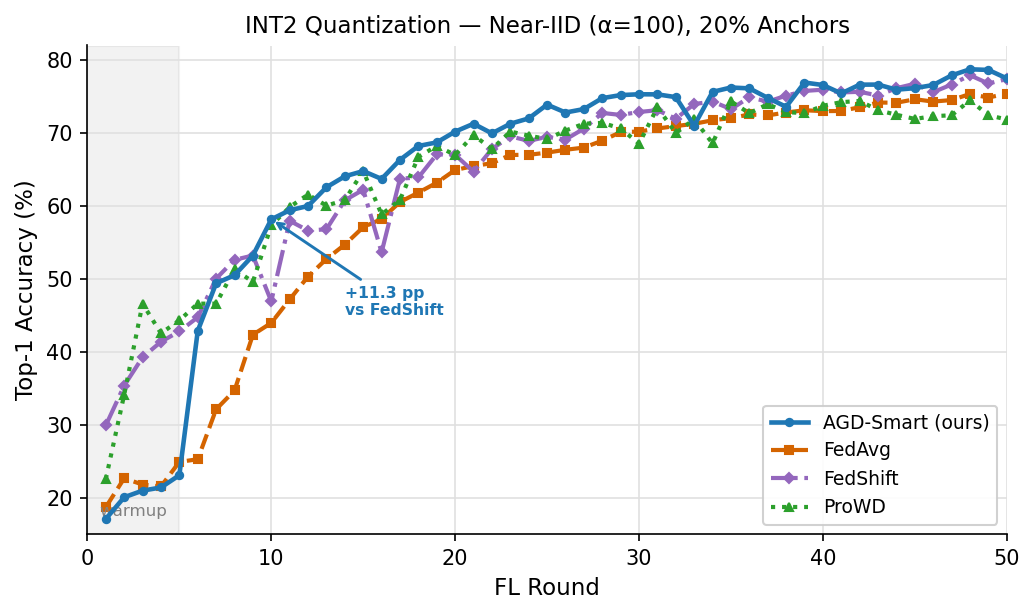
\includegraphics[width=\linewidth]{int2_curve.png}

\column{0.36\textwidth}
\footnotesize
\begin{block}{Setting}
Near-IID CIFAR-10\\
INT2 quantization, 20\% anchors\\
50 rounds
\end{block}

\textbf{FedShift / FedAvg / ProWD}
\begin{itemize}\setlength{\itemsep}{0.15em}
  \item R10: \textbf{58.2} vs 46.9 / 44.0 / 57.3
  \item R50: \textbf{77.5} vs 77.4 / 75.4 / 71.8
  \item Early edge: \textbf{+11.3} over FedShift
\end{itemize}
\end{columns}
\end{frame}

\begin{frame}{Why INT2 Is the Threshold}
\begin{columns}[T,totalwidth=\textwidth]
\column{0.56\textwidth}
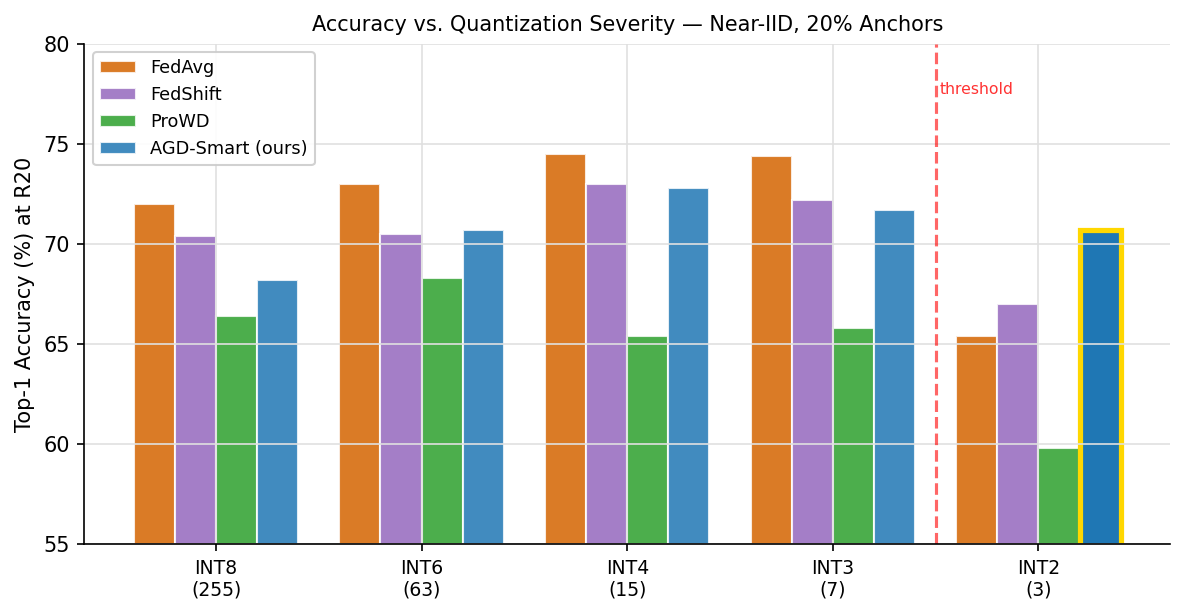
\includegraphics[width=0.88\linewidth]{noise_scaling.png}

\column{0.40\textwidth}
\footnotesize
\textbf{Key observation}
\begin{itemize}
  \item AGD-Smart only beats FedAvg once quantization becomes too coarse for averaging to recover the signal.
\end{itemize}

\vspace{0.3em}
\textbf{Why INT2 is different}
\begin{itemize}
  \item Only \textbf{3 effective levels}: negative, zero, positive.
  \item Large and small gradients collapse to the same code.
  \item Opposite signs cancel across clients.
\end{itemize}

\vspace{0.3em}
\textbf{Interpretation}
\begin{itemize}
  \item At INT3 and above, FedAvg usually has enough resolution to survive.
  \item At INT2, the learned correction becomes genuinely useful.
\end{itemize}
\end{columns}
\end{frame}

\begin{frame}{FedShift Comparison at Round 50}
\small
\begin{center}
\resizebox{0.92\linewidth}{!}{%
\begin{tabular}{lccccc}
\toprule
Setting & FedAvg & FedShift & ProWD & AGD-Smart \\
\midrule
Near-IID, INT2 & 75.4 & 77.4 & 71.8 & \textbf{77.5} \\
Near-IID, INT8 & \textbf{82.7} & 81.1 & 79.3 & 81.2 \\
Near-IID, INT4 & \textbf{83.2} & 80.7 & 77.7 & 82.5 \\
Non-IID, INT8  & \textbf{80.4} & 73.8 & 72.8 & 74.8 \\
\bottomrule
\end{tabular}}
\end{center}

\vspace{0.6em}
\begin{block}{Interpretation}
This view is easier to read because it shows the actual endpoints. FedShift is
usually stronger than ProWD, which makes it the more serious correction
baseline, but AGD-Smart still recovers the best corrected score in INT2, INT4,
and non-IID INT8. FedAvg remains strongest in the easier INT8 and INT4
near-IID settings.
\end{block}
\end{frame}

\begin{frame}{Where AGD-Smart Beats FedShift}
\begin{center}
\resizebox{0.92\linewidth}{!}{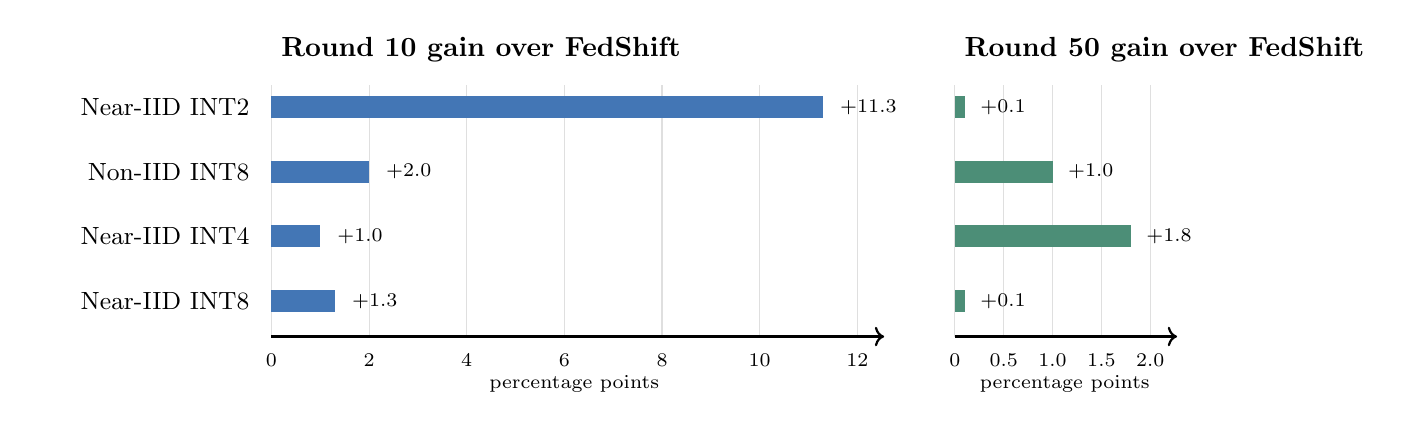
\begin{tikzpicture}[x=0.62cm,y=0.82cm,font=\small]
  \def\barhalf{0.17}

  \node[anchor=west,font=\bfseries] at (0,4.9) {Round 10 gain over FedShift};
  \node[anchor=west,font=\bfseries] at (14,4.9) {Round 50 gain over FedShift};

  \foreach \x/\lab in {0/0,2/2,4/4,6/6,8/8,10/10,12/12} {
    \draw[gray!25] (\x,0.45) -- (\x,4.35);
    \node[font=\scriptsize] at (\x,0.08) {\lab};
  }
  \draw[->,thick] (0,0.45) -- (12.55,0.45);
  \node[font=\scriptsize] at (6.2,-0.28) {percentage points};

  \foreach \x/\lab in {14/0,15/0.5,16/1.0,17/1.5,18/2.0} {
    \draw[gray!25] (\x,0.45) -- (\x,4.35);
    \node[font=\scriptsize] at (\x,0.08) {\lab};
  }
  \draw[->,thick] (14,0.45) -- (18.55,0.45);
  \node[font=\scriptsize] at (16.25,-0.28) {percentage points};

  \foreach \y/\name/\early/\final in {
    4/{Near-IID INT2}/11.3/0.1,
    3/{Non-IID INT8}/2.0/1.0,
    2/{Near-IID INT4}/1.0/1.8,
    1/{Near-IID INT8}/1.3/0.1
  } {
    \node[anchor=east,align=right,text width=2.7cm] at (-0.25,\y) {\name};
    \fill[anchorblue!85] (0,\y-\barhalf) rectangle (\early,\y+\barhalf);
    \node[anchor=west,font=\scriptsize] at (\early+0.15,\y) {+\early};
    \pgfmathsetmacro{\finalx}{14 + 2*\final}
    \fill[buffergreen!85] (14,\y-\barhalf) rectangle (\finalx,\y+\barhalf);
    \node[anchor=west,font=\scriptsize] at (\finalx+0.12,\y) {+\final};
  }
\end{tikzpicture}
}
\end{center}

\vspace{0.3em}
\small
\begin{itemize}
  \item INT2 is the early-convergence story: AGD-Smart is up \textbf{+11.3} at round 10 even though the final scores nearly tie.
  \item INT4 is the clearest end-of-training story: AGD-Smart finishes \textbf{+1.8} ahead.
  \item Non-IID INT8 shows why smart matching matters: a single global shift is too coarse once client distributions diverge.
\end{itemize}
\end{frame}

\begin{frame}{Other Regimes}
\begin{columns}[T,totalwidth=\textwidth]
\column{0.32\textwidth}
\begin{block}{Near-IID, INT8}
\footnotesize
AGD-Smart reaches \textbf{81.2} at R50, essentially ties FedShift at 81.1, and
still trails FedAvg slightly at the end.
\end{block}

\column{0.32\textwidth}
\begin{block}{Near-IID, INT4}
\footnotesize
AGD-Smart reaches \textbf{82.5} at R50, beats FedShift by \textbf{+1.8}, and
finishes within 0.7 of FedAvg.
\end{block}

\column{0.32\textwidth}
\begin{block}{Non-IID, INT8}
\footnotesize
AGD-Smart reaches \textbf{74.8} at R50, beats FedShift by \textbf{+1.0}, but
FedAvg still benefits from preserving client diversity.
\end{block}
\end{columns}

\vspace{0.6em}
\small
\begin{center}
Across the shared settings, the stable pattern is:
\textbf{AGD-Smart $\geq$ FedShift $>$ ProWD} under near-IID data, while
\textbf{AGD-Smart $>$ FedShift} is more meaningful under INT4, INT2 early
rounds, and non-IID data.
\end{center}
\end{frame}

\begin{frame}{Takeaways}
\begin{block}{What the method is doing}
It uses clean anchor-client updates to supervise a persistent server-side
corrector for low-bit client deltas.
\end{block}

\begin{block}{Why it beats ProWD and often FedShift}
\begin{itemize}
  \item replayed supervision instead of round-by-round forgetting,
  \item client-specific smart matching instead of a single mean target,
  \item warmup and blending so correction turns on more safely.
\end{itemize}
\end{block}

\begin{alertblock}{Main conclusion}
This is not a universal replacement for FedAvg. It is a targeted fix for the
regime where quantization is severe enough that averaging alone fails, and it
stays most convincing when a simple global shift is not enough, especially
INT2 early and non-IID data.
\end{alertblock}
\end{frame}

\begin{frame}{Selected References}
\footnotesize
\begin{itemize}
  \item McMahan et al. (2017), \emph{Communication-Efficient Learning of Deep Networks from Decentralized Data}.
  \item Li et al. (2020), \emph{Federated Optimization in Heterogeneous Networks}.
  \item Karimireddy et al. (2020), \emph{SCAFFOLD: Stochastic Controlled Averaging for Federated Learning}.
  \item Wang et al. (2020), \emph{Tackling the Objective Inconsistency Problem in Heterogeneous Federated Optimization}.
  \item Reisizadeh et al. (2020), \emph{FedPAQ: A Communication-Efficient Federated Learning Method with Periodic Averaging and Quantization}.
  \item Yoon et al. (2022), \emph{Bitwidth Heterogeneous Federated Learning with Progressive Weight Dequantization}.
  \item Seo et al. (2024), \emph{FedShift: Robust Federated Learning Aggregation Scheme in Resource Constrained Environment via Weight Shifting}.
  \item Chen and Vikalo (2024), \emph{Mixed-Precision Quantization for Federated Learning on Resource-Constrained Heterogeneous Devices}.
\end{itemize}
\end{frame}

\begin{frame}[plain]
  \vfill
  \begin{center}
    {\LARGE\bfseries Questions?}
  \end{center}
  \vfill
\end{frame}

\end{document}
